\chapter{Resultat}

Som kvalitetskontrol for client/server systemet skal den overførte fil kunne
sammenlignes med den oprindelige fil vha. terminal-kommandoen:
cmp <afsendt fil> < modtaget fil>
eller
diff –s <afsendt fil> < modtaget fil>
<afsendt fil> er overført til client vha. af email, ftp eller anden pålidelig, ikke
proprietær overføringsmetode.
Der må ikke være forskel mellem filerne, hverken mht. til størrelse eller mht. indhold.

\section{Udførelse}

Som det fremgår af figur \ref{fig:file_serverTCP} og \ref{fig:file_clientTCP}, overfører vi en fil, som det er forespurgt i opgaveformuleringen. 
I vores tilfælde overføres et billede der hedder "Batman.jpg". Til at sammenligne, har vi samme fil, som skal overføres, liggende i clientmappen som "Original\_Batman.jpg". 

Koden udskriver info til brugeren om overførslens forløb, samt størrelsen af den overførte fil. 

\begin{figure}[h!]
	\centering
	\fbox{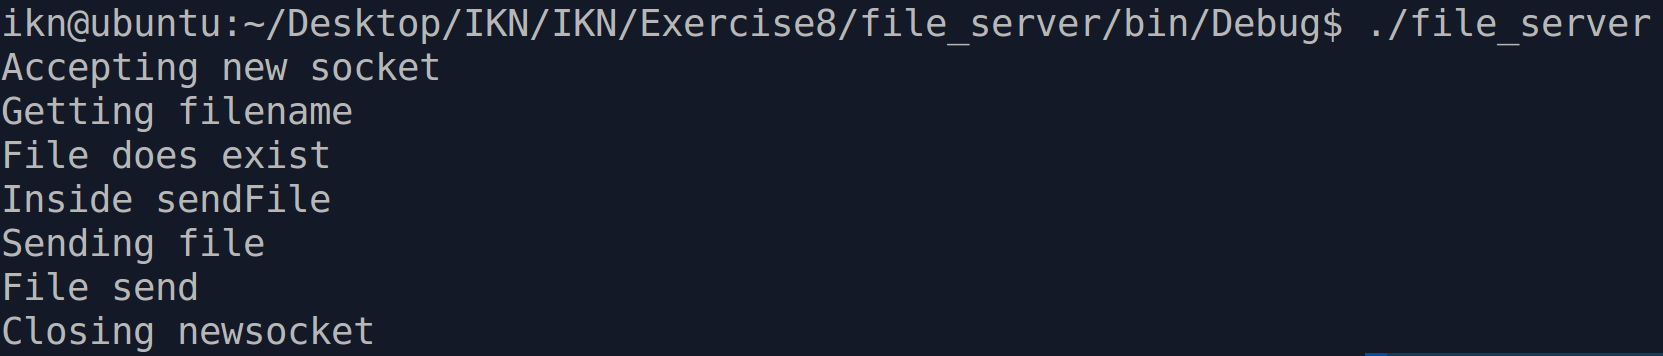
\includegraphics[scale=0.5]{Pic/file_server}}
	\caption{TCP-overførsel på server-siden}
	\label{fig:file_serverTCP}
\end{figure}


\begin{figure}[h!]
	\centering
	\fbox{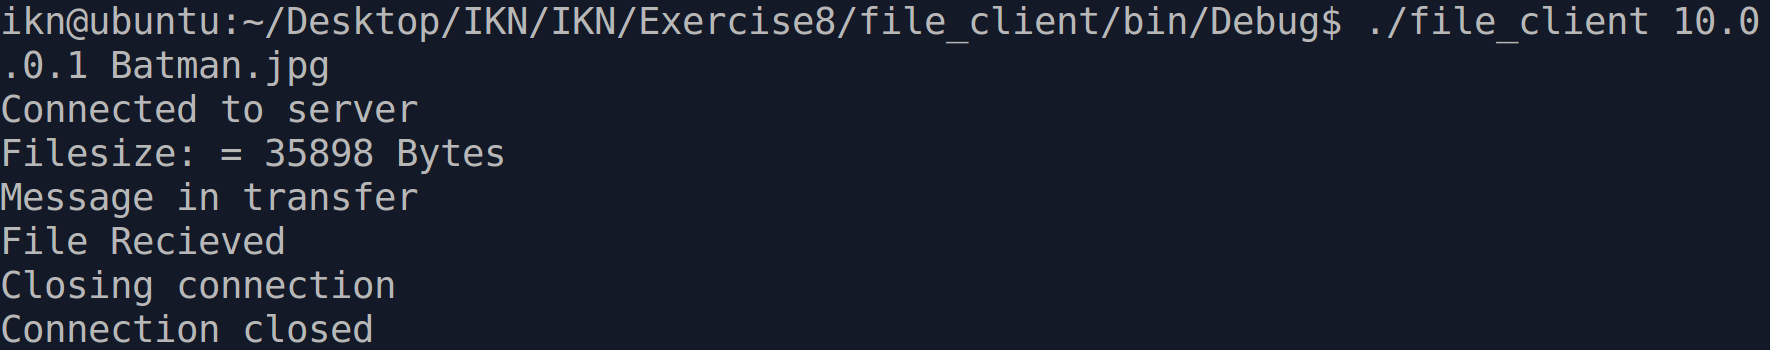
\includegraphics[scale=0.5]{Pic/file_client}}
	\caption{TCP-overførsel på klient-siden}
	\label{fig:file_clientTCP}
\end{figure}

 Afslutningsvist udføres en sammenligning af filerne, for at tjekke at overførslen er udført korrekt og uden fejl. I figur \ref{fig:compare}  benyttes dog kommandoen \textit{diff - s} til sammenligning, da \textit{cmp} ikke giver andet feedback, end at den afsluttes uden fejlbeskeder. 
 
 \begin{figure}[h!]
 	\centering
 	\fbox{\includegraphics[scale=0.5]{Pic/compare}}
 	\caption{Sammenligning af den overførte fil, med originalen}
 	\label{fig:compare}
 \end{figure}